\section{Software}
	\label{sec:software}
	As stated in the introduction, one of the core aims of this dissertation project was to create software that enabled novice users as well as developers to optimise the placement of wireless nodes in 2D environments. The process by which this was done, the technologies that were used and the products of this process are detailed here. 
	
	The code is available at \url{https://git.james.gg/WNP}.
	
	\subsection{Development Process}
		\label{sec:software_dev_process}
		Our development process loosely followed Agile principles \cite{agilemanifesto}. The creation of the optimisation library and the interfaces that used them were done jointly so that both pieces of software could inform how the other would be used and what data would be necessary to share between the two. This was done in a rapid iteration process by which minimum viable products (MVPs) were produced to a specification whilst keeping the codebase general enough to allow for future modification. 
	
	\subsubsection{Software Stack}
		\label{sec:software_stack}
		The optimisation libraries are written in Python 3 with little use of non-standard libraries save for the gaussian process regressor for bayesian optimisation, provided by `scikit-learn'\cite{pedregosa2011scikit} (a machine learning library for Python) and some standard data science libraries like numpy\cite{numpy2020}.

		There are several aspects of Python that make it particularly suited to this project's goals. First class function support is a feature that allows for functions to be stored in variables and passed from one section of code to another. This allows the optimisation library to have the techniques be defined more broadly and take a function as an input variable to be repeatedly called during execution. Scientific library support for Python is another key draw. Libraries such as numpy, matplotlib\cite{hunter2007matplotlib} and scikit-learn are fast and compatible, offering a great deal of support for the reshaping of arrays, drawing graphs for the GUI and access to Gaussian Process Regressors respectively.

		The command line interface is written in pure Python and provides textual output that acknowledges the input files, declares their properties and then runs all of the optimisers. The code is very simple and can easily be modified to support other functionality or additional data output.

		The graphical user interface is also written in Python and uses PySide6, a Qt library for Python and matplotlib. Qt is a GUI toolkit for creating cross-platform GUIs, which was ideally suited to our application as we didn't want to limit platforms it may run on. Matplotlib is a Python library that allows for the drawing of graphs entirely in Python code and it is used to draw the outputs of the optimisations. The produced software can run on any platform that Python can run on, as long as the required libraries and the Python runtime are installed on the host machine.

		Testing was carried out using Python's `unittest' library. Using unit tests we could ensure that newly written code conformed to expected specifications and outputs were correctly formed in a similar fashion to `continuous deployment'\cite{shahin2017deployment}.

		We used git\cite{gitscm} to track our work. This allowed me to refer to previous versions of our code and experiment freely without worrying about losing past progress. Git's branch feature was also used heavily so that a main branch with a working product could be preserved whilst experimentation took place.

	\subsection{Bounds Object and File Format}
		\label{sec:software_bounds}
		As discussed in the introduction of chapter \ref{sec:traditional}, we need access to a few key pieces of external data in order to give our optimisation algorithm a meaningful chance at success. Some of these pieces of data are obvious -- for example, each dimension will have an upper bound and a lower bound. If an algorithm does not have access to this information, it will have no clue within what space it is allowed to operate, which neighbours it may move to (in the case of simulated annealing). Many of the queries it produces would simply be wrong. Additionally, information such as the number of iterations will often inform the weight that one action is assigned over another.
		
		To ensure that all the techniques that have been implemented have access to the same data, we have designed a simple object and file format called .bounds. This object and file format stores all basic and necessary information about the environment in which we are seeking to place nodes. This includes the size of the room, which is assumed to start at $0, 0$, a name, the number of iterations or objective function queries we allow, whether we are minimising or not, constraints concerning where nodes can be placed, the number of wireless nodes we are allowed to place and the points in the room that we are seeking to cover.

		The simple interfaces that accompany the optimisation libraries also include basic warnings about perceived abnormalities in bounds files. If the bounds file specifies fewer or an equal number of points of interest than nodes to be placed, the interfaces will provide the advice that a reduced number of wireless nodes may be more economical.
		
		\lstinputlisting[label={lst:warning}, caption={The output from the command line interface warning the user about inefficient use of nodes.}]{./listings/cli_warning.txt}
		
		See a full example bounds file at appendix \ref{app:bounds}. Parsing these files is simple and an example of doing so in Python is provided in the $from\_file$ method in $bounds.py$.

	\subsection{Command Line Interface}  
		\label{sec:software_cli} 
		The command line interface was developed to allow developers or users working in headless environments to quickly make use of the optimisation library without having to read and understand the code in any great detail.

		The textual output of this interface is easy to read and understand and could be consumed by another program from an output file or a UNIX pipe if Python bindings are not available in whatever chosen language the other program is using.

	\subsection{Graphical User Interface} 
		\label{sec:software_gui} 
		The graphical user interface was developed to allow more novice users access to the optimisation library by presenting the results of an optimisation in an easy to understand format with the use of matplotlib graphs demonstrating a two-dimensional sample of the function space.

		\begin{figure}[H]
		\centering
		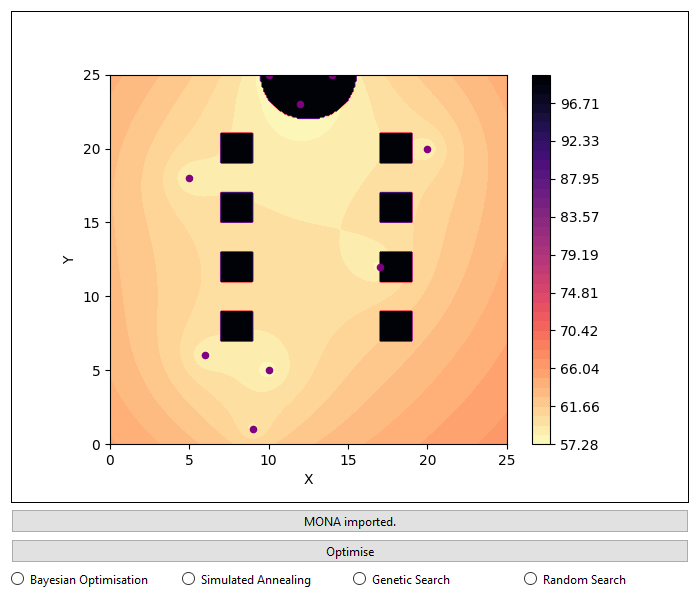
\includegraphics[scale=0.75]{graphics/gui}
		\caption{WNP GUI}
		\label{fig:gui}
		\end{figure}

		Figure \ref{fig:gui} shows a basic result. The floor plan can be seen along with the constraints, the points we are attempting to optimise around with their free space path loss shown as heat maps that gradually reduce as the distance increases.
		
	\subsection{Testing}
		\label{sec:software_testing}
		Below are some abbreviated test suites that describe the fulfilment of the objectives given in chapter \ref{sec:intro}.
		\subsubsection{User Acceptance}
			\label{sec:software_acceptance}
			User acceptance testing guarantees that the command line interface and the graphical user interface are working as expected. \\
			\begin{center}
				\small
				\begin{tabular}{| p{5cm} | p{1.5cm} | p{5cm}|}
				\hline
				\textbf{Test Description} & \textbf{Pass or Fail} & \textbf{Contribution} \\
				\hline
				CLI: The specified bounds file is imported and its properties are displayed. & Pass & Users can specify bounds files to import through command line arguments. \\
				\hline
				CLI: The optimisations are run and their outputs are displayed. & Pass & Users receive the output of the traditional and novel optimisation techniques. \\
				\hline
				GUI: Bounds files are imported and their layout is displayed. & Pass & Users are shown their bounds file as a heat map graph. \\
				\hline
				GUI: Optimisation techniques can be chosen and their result is displayed. & Pass & Users are shown the output of their chosen optimisation technique on the aforementioned heat map graph. \\
				\hline
				\end{tabular}
			\end{center}
				
		\subsubsection{Unit Testing}
			\label{sec:software_unit}
			The unit test suite exists to ensure that changes to the codebase do not adversely affect the running of the software. \\
			\begin{center}
				\small
				% \begin{longtable}{| p{5cm} | p{2cm} | p{2cm} |}
				% 	\hline
				% 	\textbf{Test Suite} & \textbf{Test Count} & \textbf{Tests Passed} \\
				% 	\hline
				% 	Bounds Test Suite & 10 & 10 \\
				% 	\hline
				% 	Search Test Suite & 4 & 4 \\
				% 	\hline
				% \end{longtable}
			\end{center}